\documentclass[12pt,english]{article}
\usepackage[utf8]{inputenc}
\usepackage{geometry}
\usepackage{graphicx}
\usepackage{mathtools}
\usepackage{setspace}
\usepackage{siunitx}
\usepackage{minted}
\usepackage{todonotes}
\geometry{
a4paper,
left=25mm,
right=25mm,
top=25mm,
bottom=25mm,
}
\usepackage{babel}
\usepackage{lmodern}
\usepackage[T1]{fontenc}
\usepackage{float}
\usepackage{tikz}
\usepackage{pgfplots}
\pgfplotsset{compat=newest}
\usepgfplotslibrary{units}
\usepackage{standalone}
\usepackage{tikzscale}
\makeatletter
\pgfplotsset{
  unit code/.code 2 args=
    \begingroup
    \protected@edef\x{\endgroup\si{#2}}\x
}
\makeatother
\renewcommand{\baselinestretch}{1.1} 
\newcommand{\Hvec}{\vec{H}}
\newcommand{\Evec}{\vec{E}}
\renewenvironment{cases}
{ \left\{\begin{aligned} }
{ \end{aligned}\right. }
\renewcommand{\epsilon}{\varepsilon}
\usepackage[hidelinks]{hyperref}

\begin{document}

\begin{titlepage}
	{\setstretch{1.0}


\includegraphics[width=\textwidth]{img/Logos.pdf} \hspace{4.5cm}

\vspace{1 cm}
\large

\begin{tabular}{lr}
\begin{minipage}[t]{0.5\textwidth}
{\small\textsc{Brussels Faculty of Enginering} \\[1ex]
Université Libre de Bruxelles\\[1ex]
Vrije Universiteit van Brussel\\[1ex]}
\end{minipage} & \begin{minipage}[t]{0.45\textwidth}
\begin{flushright}
{\small Academic Year 2016-2017}
\end{flushright}
\end{minipage}
\end{tabular}

\vspace{\stretch{2}}
\begin{center}
\Large 
\textbf{Project Report} \\Numerical resolution of the Maxwell equations using the Finite-Difference Time-Domain method\\
\vspace{3 cm}
\large
Victor Artois, Cédric Hannotier, Mathieu Petitjean\\ 
\end{center}


\vspace{\stretch{2}}

\begin{minipage}[t]{\textwidth}
\normalsize \textbf{ELEC-H415}: Communication Channels\\[1.5ex]
\end{minipage}
}

\end{titlepage}
\thispagestyle{empty}
\tableofcontents
\newpage
%\thispagestyle{plain}
\setcounter{page}{1}
\section{Introduction}
This report presents the derivation and implementation of a two dimensional finite-difference time-domain (FDTD) algorithm for the resolution of the Maxwell equations. 

First, the Maxwell equations are discretized in order to obtain implementable update equations for the fields. Then advanced boundary conditions are discussed in order to avoid reflections on the borders of the grid. Finally, the C source codes are shown, their functioning is detailed and a validation procedure is carried out.

These codes were used to illustrate the main concepts of electromagnetism presented in the Communication Channels course at the Brussels Faculty of Engineering. The derivation of the equations as well as the codes are based on the works of John Schneider\footnote{Understanding the FDTD method: \url{http://www.eecs.wsu.edu/~schneidj/ufdtd/}\label{fn}}.

\iffalse
\section{Simulation ideas}
\begin{itemize}
    \item Fast-fading: simulate a $500\times500$ metallic box and analyze power repartition in various 30x30 regions (see statement).
    \item Check the Friis free-space attenuation in $\frac{\lambda}{d^2}$ (chap 2).
    \item Build a knife-edge model and verify that ${\left | F(\nu) \right |}^2 \sim \frac{1}{2 \pi ^2 \nu ^2}$ (chap 3).
    \item Body Area Network: study the propagation of waves around the human body for various frequencies.
    \item Check the validity of the assumption that free-space attenuation can be considered if 60\% of the Fresnel ellipsoid is free of any obstacle (chap 5).
    \item Build an array of 4 dipole antennas and observe beam forming (chap 6).
    \item Build a panel antenna and observe radiation pattern (chap 6).
    \item Build a parabolic antenna and visualize emission (chap 6).
    \item Simulate propagation inside of a dielectric slab (chap 9).
\end{itemize}
\fi

\section{2D FDTD algorithm}
The algorithm for the two-dimensional FDTD method is derived under the assumption of a TM$^z$ polarization (Transverse Magnetic, the magnetic field is transverse to the direction of propagation $z$). The Faraday and Ampere laws can be written:

\begin{equation}
\begin{cases}
	-\sigma_m\Hvec -\mu \frac{\partial \Hvec}{\partial t} &=
	\nabla \times \Evec	\\
	\sigma \Evec + \epsilon \frac{\partial \Evec}{\partial t} &=
	\nabla \times \Hvec
\end{cases}	
\label{eq:maxwell}
\end{equation}

Using the fact that the only non-zero elements are $E_z$, $H_x$ and $H_y$, (\ref{eq:maxwell}) can be rewritten in the set of scalar equations:

\begin{equation}
	\begin{cases}
		-\sigma_m H_x - \mu\frac{\partial H_x}{\partial t} &=
		\frac{\partial E_z}{\partial y}
		\\
		\sigma_m H_y + \mu\frac{\partial H_y}{\partial t} &=
		\frac{\partial E_z}{\partial x}
		\\
		\sigma E_z + \varepsilon\frac{\partial E_z}{\partial t} &=
		\frac{\partial H_y}{\partial x}
		-\frac{\partial H_x}{\partial y} 
	\end{cases}	
	\label{eq:scalar}
\end{equation}

These equations now need to be discretized in order to be solved numerically. First, the fields are discretized in space and time. $a$ corresponds to the spatial step in the $x$ direction, $b$ to the spatial step in the $y$ direction and $n$ corresponds to the temporal step.

\begin{equation}
    \begin{aligned}
		H_x(x,y,t) &= H_x(a\Delta x, b \Delta y, n \Delta t) \equiv
		H_x^n[a,b]  \\
		H_y(x,y,t) &= H_y(a\Delta x, b \Delta y, n \Delta t) \equiv
		H_y^n[a,b]  \\
		E_z(x,y,t) &= E_z(a\Delta x, b \Delta y, n \Delta t) \equiv
		E_z^n[a,b]
	\end{aligned}
\end{equation}

The derivative of (\ref{eq:scalar}) will then be approximated by finite differences. By neglecting second order terms in the step $\delta$, one can find:

\begin{equation}
	f'(x_0) = \frac{f\left(x_0 + \frac{\delta}{2}\right) - f\left(x_0 - \frac{\delta}{2}\right)}{\delta} + \mathcal{O}(\delta^2) \simeq \frac{f\left(x_0 + \frac{\delta}{2}\right) - f\left(x_0 - \frac{\delta}{2}\right)}{\delta}
	\label{eq:deriv}
\end{equation}

In order to use (\ref{eq:deriv}) to obtain the update equations of the field, it is necessary to include an offset between the electric and magnetic fields. The assumption is done that the electric field nodes are located on integer values of the steps while the magnetic field nodes have offsets of half a step, as shown in Figure \ref{fig:grid}.

\begin{figure}[H]
    \centering
    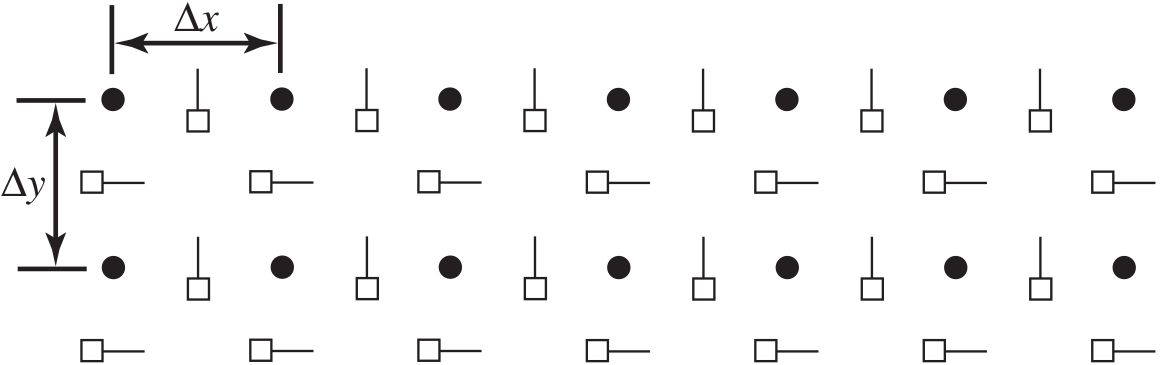
\includegraphics[width=.6\linewidth]{img/grid.png}
    \caption{Physical setup of the FDTD grid. The circles represent the electric field nodes $E$ while the squares represent the magnetic field nodes $H$. An offset of half a spatial step is present\textsuperscript{\ref{fn}}.}
    \label{fig:grid}
\end{figure}

With this particular arrangement of the nodes, the first equation of (\ref{eq:scalar}) can be expanded around the point $(x,y,t) = (a \Delta x, (b+\frac{1}{2}) \Delta y, n \Delta t)$. Each term of the equation is detailed:

\begin{equation}
	\begin{split}
	-\sigma_m H_x^n \left[a,b+\frac{1}{2}\right] &\simeq - \sigma_m \frac{H_x^{n+\frac{1}{2}}\left[a,b+\frac{1}{2}\right] + H_x^{n-\frac{1}{2}}\left[a,b+\frac{1}{2}\right] }{2}\\
	- \mu\frac{\partial H_x}{\partial t} &\simeq - \mu \frac{H_x^{n+\frac{1}{2}}\left[a,b+\frac{1}{2}\right] - H_x^{n-\frac{1}{2}}\left[a,b+\frac{1}{2}\right]}{\Delta t} \\
	\frac{\partial E_z}{\partial y} &\simeq \frac{E_z^{n}\left[a,b+1\right] - E_z^{n}[a,b]}{\Delta y}
	\end{split}
\end{equation}

In the approximated equation, the future term ($H_x$ at time step $n + \frac{1}{2}$) can be obtained from the past ones. Once isolated, it is expressed as: \vspace*{-0.7cm}

\begin{equation}
	H_x^{n+\frac{1}{2}}\left[a,b+\frac{1}{2}\right] =
	\frac{1-\frac{\sigma_m \Delta t}{2 \mu}}{1+\frac{\sigma_m \Delta t}{2 \mu}} H_x^{n-\frac{1}{2}}\left[a,b+\frac{1}{2}\right] -
	\frac{1}{1 + \frac{\sigma_m \Delta t}{2 \mu}} \frac{\Delta t}{\mu \Delta y}
	(E_z^n[a,b+1] - E_z^n[a,b])
	\label{eq:updateHx}
\end{equation}

In (\ref{eq:updateHx}), the parameters $\mu$ and $\sigma_m$ are the value of the material at the space point $(x,y) = (a \Delta x, b + \frac{1}{2} \Delta y)$. Following the same reasoning, the update equations for $H_y$ and $E_z$ can be found:

\begin{equation}
H_y^{n+\frac{1}{2}}\left[a+\frac{1}{2},b\right] =
\frac{1-\frac{\sigma_m \Delta t}{2 \mu}}{1+\frac{\sigma_m \Delta t}{2 \mu}} H_y^{n-\frac{1}{2}}\left[a+\frac{1}{2},b\right] +
\frac{1}{1 + \frac{\sigma_m \Delta t}{2 \mu}} \frac{\Delta t}{\mu \Delta x}
(E_z^n[a+1,b] - E_z^n[a,b])
\end{equation}

\begin{equation}
\begin{aligned}
E_z^{n+1}[a,b] =
\frac{1-\frac{\sigma \Delta t}{2 \epsilon}}{1+\frac{\sigma \Delta t}{2 \epsilon}} E_z^{n}[a,b] + \frac{1}{1+\frac{\sigma \Delta t}{2 \epsilon}}
\left(
\frac{\Delta t}{\epsilon \Delta x} \left\{ H_y^{n+\frac{1}{2} } \left[a + \frac{1}{2}, b\right] -  H_y^{n+\frac{1}{2} } \left[a - \frac{1}{2}, b\right] 
\right\} \right.\\
\left.- \frac{\Delta t}{\epsilon \Delta x} \left\{
H_x^{n+\frac{1}{2} } \left[a,b+ \frac{1}{2}\right] -  H_x^{n+\frac{1}{2} } \left[a, b- \frac{1}{2}\right]
\right\} \right)
\label{eq:update2}
\end{aligned}
\end{equation}

\section{Absorbing boundary conditions}
When implementing the previous update equation in a program, one needs to investigate the value assigned to the extreme values of the grid, because these cannot be updated through the update equations. For example, when computing $E_z^{n+1} \left[ 0,0 \right]$, the value $H_y^{n+\frac{1}{2}} \left[ 0 , - \frac{1}{2} \right ]$ is not available.

One basic approach is to impose the electric field to be zero on the boundaries of the grid. Physically, a region where the electric field is always zero is a perfect electric conductor. Any incoming electromagnetic wave on such a conductor will be totally reflected. This can be a wanted behaviour in some simulations, but absorbing boundaries must be implemented in order to simulate an infinite environment. 

Since the update equations cannot be used, the following reasoning is based on the wave equation that governs the propagation of the electric field:

\begin{equation}
    \left( \frac{\partial^2}{\partial x^2} - \mu \epsilon \frac{\partial ^2}{\partial t^2} \right) E_z =  \left( \frac{\partial}{\partial x} - \sqrt{\mu \epsilon} \frac{\partial}{\partial t} \right) \left( \frac{\partial}{\partial x} + \sqrt{\mu \epsilon} \frac{\partial}{\partial t} \right)E_z = 0
\end{equation}

This equation will be discretized around the point $(x,t) = \left(\frac{\Delta x}{2}, (n+\frac{1}{2}) \Delta t\right)$. The electrical field was defined on integer values of spatial indexes, so that $E_z^n\left[\frac{1}{2}\right]$ will be approximated by $(E_z^n\left[0\right] + E_z^n\left[1\right])/2$. In the following equations, a compact notation has been introduced for readability. $I$ denotes the identity operator, $\sigma_t$ is a time shift and $\sigma_x$ is a spatial shift.

\begin{equation}
	\left.\frac{\partial E_z}{\partial t}\right|_{\left(\frac{\Delta x}{2}, (n+\frac{1}{2}) \Delta t\right)} = \frac{\frac{E_z^{n+1} \left[0\right] + E_z^{n+1} \left[1\right]}{2} - \frac{E_z^{n} \left[0\right] + E_z^{n} \left[1\right]}{2}}{\Delta t} =  \left( \frac{I - \sigma_t^{-1}}{\Delta t} \right) \left( \frac{I + \sigma_x^{1}}{2}\right) E_z^{n+1} \left[0\right]	
\end{equation}

\begin{equation}
\left.\frac{\partial E_z}{\partial x}\right|_{\left(\frac{\Delta x}{2}, (n+\frac{1}{2}) \Delta t\right)} = \frac{\frac{E_z^{n+1} \left[1\right] + E_z^{n} \left[1\right]}{2} - \frac{E_z^{n+1} \left[0\right] + E_z^{n} \left[0\right]}{2}}{\Delta x} =  \left( \frac{\sigma_x^{1} - I}{\Delta x} \right) \left( \frac{I + \sigma_t^{-1}}{2}\right) E_z^{n+1} \left[0\right]	
\end{equation}

The wave equation can thus be rewritten in operator form, and the advection operator $\boldsymbol{A}$ is defined.

\begin{equation}
	\left \{
	\left( \frac{\sigma_x^{1} - I}{\Delta x} \right) \left( \frac{I + \sigma_t^{-1}}{2}\right)  - \sqrt{\mu \epsilon}\left( \frac{I - \sigma_t^{-1}}{\Delta t} \right) \left( \frac{I + \sigma_x^{1}}{2}\right)
	\right\} E_z^{n+1} \left[0\right] = \boldsymbol{A} E_z^{n+1}[0] = 0
	\label{eq:abc1}
\end{equation}

The update equation provided by (\ref{eq:abc1}) is approximate. Better results are obtained when using a second order equation, which means that the advection operator is applied twice. This way, a long but often accurate update equation can be deduced.

\begin{equation}
	\boldsymbol{A} \boldsymbol{A} E_z^{n+1} = 0
\end{equation}

\begin{equation}
\begin{aligned}[rl]
	E_z^{n+1} \left[0\right] = &\frac{-1}{1/S_c^{'} + 2 + S_c^{'}} \{ (1/S_c^{'} - 2 + S_c^{'}) \left[ E_z^{n+1} \left[2\right] + E_z^{n-1} \left[0\right] \right]  \\
	 & + 2 ( S_c^{'} - 1/ S_c^{'}) \left[ E_z^{n} \left[0\right]  + E_z^{n} \left[2\right] - E_z^{n+1} \left[1\right] - E_z^{n-1} \left[1\right]\right] \\
	 & -4 (1/S_c^{'} + S_c^{'}) E_z^{n} \left[1\right] \} - E_z^{n-1} \left[2\right]
\end{aligned}
\label{eq:abc2}
\end{equation}

The update equation (\ref{eq:abc2}) is expressed as a function of $S_c^{'} = \Delta t / (\sqrt{\mu \epsilon} \Delta x) = S_c /\sqrt{\mu_r \epsilon_r} $, where $S_c = c \Delta t / \Delta x$ is the Courant number. The boundary equation was derived here for the left boundary of the grid but can be similarly found for each boundary. Being a second order equation, two spatial samples are needed as well as samples that are two time steps old. This is to be taken into account during the implementation, where such samples should be stored in memory.

\section{Harmonic source}
A harmonic source can be simulated by imposing the value of the electrical field where it is located. The harmonic source equation is:
\begin{equation}\label{eq:hsource:hsource}
    E_z(t) = \cos(\omega t)
\end{equation}
In free space, $\omega$ can be rewritten as $\frac{2\pi c}{\lambda}$. To be able to implement the source in a discrete way, \eqref{eq:hsource:hsource} has to be written as a function of the spatial and temporal steps. Hence
\begin{equation}\label{eq:hsource:nlambda}
    \lambda = N_\lambda \Delta x\qquad \qquad t=n\Delta t
\end{equation}
$N_\lambda$ being the \emph{number of points per wavelength}. Using \eqref{eq:hsource:nlambda}, the harmonic source equation becomes
\begin{align}
    E_z^n &= \cos\left(\frac{2\pi c\Delta t}{N_\lambda \Delta x}n\right) \label{eq:hsource:hdelta}\\
    &= \cos\left(\frac{2\pi S_c}{N_\lambda}n\right) \label{eq:hsource:hsc}
\end{align}

Equation \eqref{eq:hsource:hsc} will be used instead of \eqref{eq:hsource:hdelta} to make it independent of $\Delta x$ and $\Delta t$.


\section{Implementation}
\subsection{Stability}\label{subsec:im:stab}
In order to guarantee the FDTD stability in 2D, a restriction on $\Delta t$ has to be done:
\begin{equation}\label{Screstrict}
    \Delta t \leq \frac{\Delta x}{c\sqrt{2}}
\end{equation}
Equation \eqref{Screstrict} can be interpreted as the impossibility of propagating the energy at more than one spatial step by time step.

To ensure FDTD stability whatever the simulation, $\Delta x$ and $\Delta t$ will not be explicitly defined. Instead, the ratio between them $S_c$ is used. Hence, $S_c=\frac{1}{\sqrt{2}}$.

\subsection{Main loop}

The main loop of the code is shown below. All functions are initialized, then the time stepping is performed.
{\setstretch{0.75}
\inputminted{c}{codes/tmzdemo1.c}}

\subsection{Fields update}\label{sec:codefields}

The following code updates the fields of the grid at each iteration, using equations (\ref{eq:updateHx}) to (\ref{eq:update2}).

{\setstretch{0.75}
\inputminted{c}{codes/updatetmz.c}}

The coefficients used in the previous code were initialised as arrays in the function \texttt{gridInit}. A shorthand notation is used: for example, \texttt{Chxh} is the coefficient multiplying $H$ when updating $H_x$.

{\setstretch{0.75}
\inputminted{c}{codes/gridtmz.c}}

\subsection{Absorbing boundary conditions}

The following code performs the update equation (\ref{eq:abc2}) at the boundaries of the grid. First, macros are defined to easily access the stored values of the field and the coefficients are computed in the initialisation function. At each iteration, the new values of the field are computed and then stored in order to perform the next computation.

{\setstretch{0.75}
\inputminted{c}{codes/abctmz.c}}

\subsection{Harmonic source}

The value of the electric field on the points where an harmonic source is present is imposed by the following code, according to Equation \ref{eq:hsource:hsc}.

{\setstretch{0.75}
\inputminted{c}{codes/harmonic.c}}

\section{Validation}
Once the theoretical update equations are implemented, a validation procedure is needed to confirm the legitimacy of the simulations. The code is validated with a test including a lossy region at the right side of the grid, while the left side is loss-less. In this case, the layer is composed of cerebral tissue (relative permittivity $\varepsilon_r$, conductivity $\sigma$) and the source of excitation is an harmonic source at frequency $f$ (this validation will be a first step to introduce the SAR simulation). The values of the parameters are summarised in \autoref{tab:valpar}. The simulation will be considered valid if the wavelength and the attenuation in the lossy layer match the expected theoretical results.

%The validation criteria will be on the verification of the wavelength value and the loss characteristic in the layer.

\begin{table}[H]
    \centering
    $\begin{array}{|c|c|}
    \hline
    \varepsilon_r & 43 \\\hline
    \sigma & \SI{1.3}{\siemens\per\meter}\\\hline
    f & \SI{915}{\mega\hertz}\\\hline
    \end{array}$
    \caption{Validation parameters}
    \label{tab:valpar}
\end{table}

The wavelength in the lossy layer is defined as
\begin{equation}
\label{eq:valid:lambdal}
    \lambda_l = \frac{v_\varphi}{f}\quad\text{where}\quad\begin{cases*}
    v_\varphi & propagation/phase velocity \\
    f & wavelength frequency
    \end{cases*}
\end{equation}
Knowing that 
\begin{equation}\label{eq:valid:vandB}
v_\varphi=\frac{\omega}{\beta}\quad\text{and}\quad \beta=\omega\sqrt{\frac{\mu_0\varepsilon_r\varepsilon_0}{2}\left[\sqrt{1+\left(\frac{\sigma}{\omega\varepsilon_r\varepsilon_0}\right)^2}+1\right]}
\end{equation}
by coupling \eqref{eq:valid:lambdal} and \eqref{eq:valid:vandB}, one finds $\lambda_l\approx\SI{48}{\milli\meter}$. Being the wavelength of interest, $\Delta x=\frac{\lambda_l}{10}=\SI{4.8}{\milli\meter}$ and $\Delta t=S_c\frac{\Delta x}{c}\approx\SI{11.32}{\nano\second}$.  

The loss can be characterised by the skin depth $\delta = \frac{1}{\alpha}$, where

\begin{equation}
\alpha = \omega\sqrt{\frac{\mu_0\varepsilon_r\varepsilon_0}{2}\left[\sqrt{1+\left(\frac{\sigma}{\omega\varepsilon_r\varepsilon_0}\right)^2}-1\right]}
\end{equation}

$\alpha$ representing the rate of decay of the wave amplitude (represented \autoref{fig:valid:alphaeg}). In that way, $\alpha\approx\SI{35.91}{\per\meter}$ and $\delta\approx\SI{2.79}{\centi\meter}$.

\begin{figure}[H]
\centering
    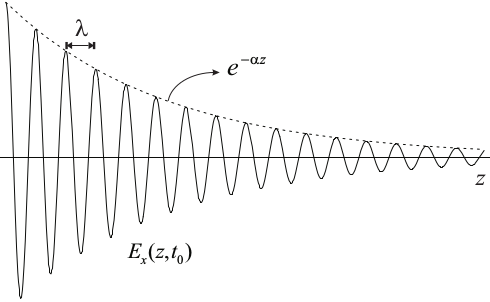
\includegraphics[width=.7\textwidth]{img/alpha}
     \caption{Decay of the wave amplitude in a lossy layer}
     \label{fig:valid:alphaeg}
\end{figure}

The different parameters needed to run the simulation are then defined, such as the number of point per wavelength $N_\lambda$ (source excitation) and the loss parameter used in the code of \autoref{sec:codefields} (equals to $\frac{\sigma\Delta t}{2\varepsilon}$ since the magnetic effects are neglected ($\sigma_m=0$, $\mu_r= 1$)).

\begin{equation}
N_\lambda=\frac{\lambda}{\Delta x} = \frac{c}{f\Delta x} \approx \num{68.20}
\end{equation}
\begin{equation}
\text{LOSS} = \frac{\pi}{N_\lambda}S_c\sqrt{\left(1+\frac{N_\lambda^2}{2\pi^2N_L^2\varepsilon_r\mu_r}\right)^2 +1} \approx\num{19.35e-3}
\end{equation} 
where
\begin{equation}
N_L = \frac{\delta}{\Delta x}
\end{equation}

The result of the simulation is shown in \autoref{fig:valid:SAR_Layer}. The electric field after the lossy layer on a horizontal line $E_z(x,100,t')$ is shown in  \autoref{fig:valid:SAR_Layer_x}. On \autoref{fig:valid:SAR_Layer_x}, the \emph{Curve Fitting} MATLAB tool was used to fit the exponential decay. $\lambda_l$ and $\alpha$ can be deduced: $\lambda_l\approx\SI{48}{\milli\meter}$ and $\alpha\approx \SI{35.26}{\per\meter}$, as expected (neglecting graphical fitting errors).

\begin{figure}[H]
\centering
    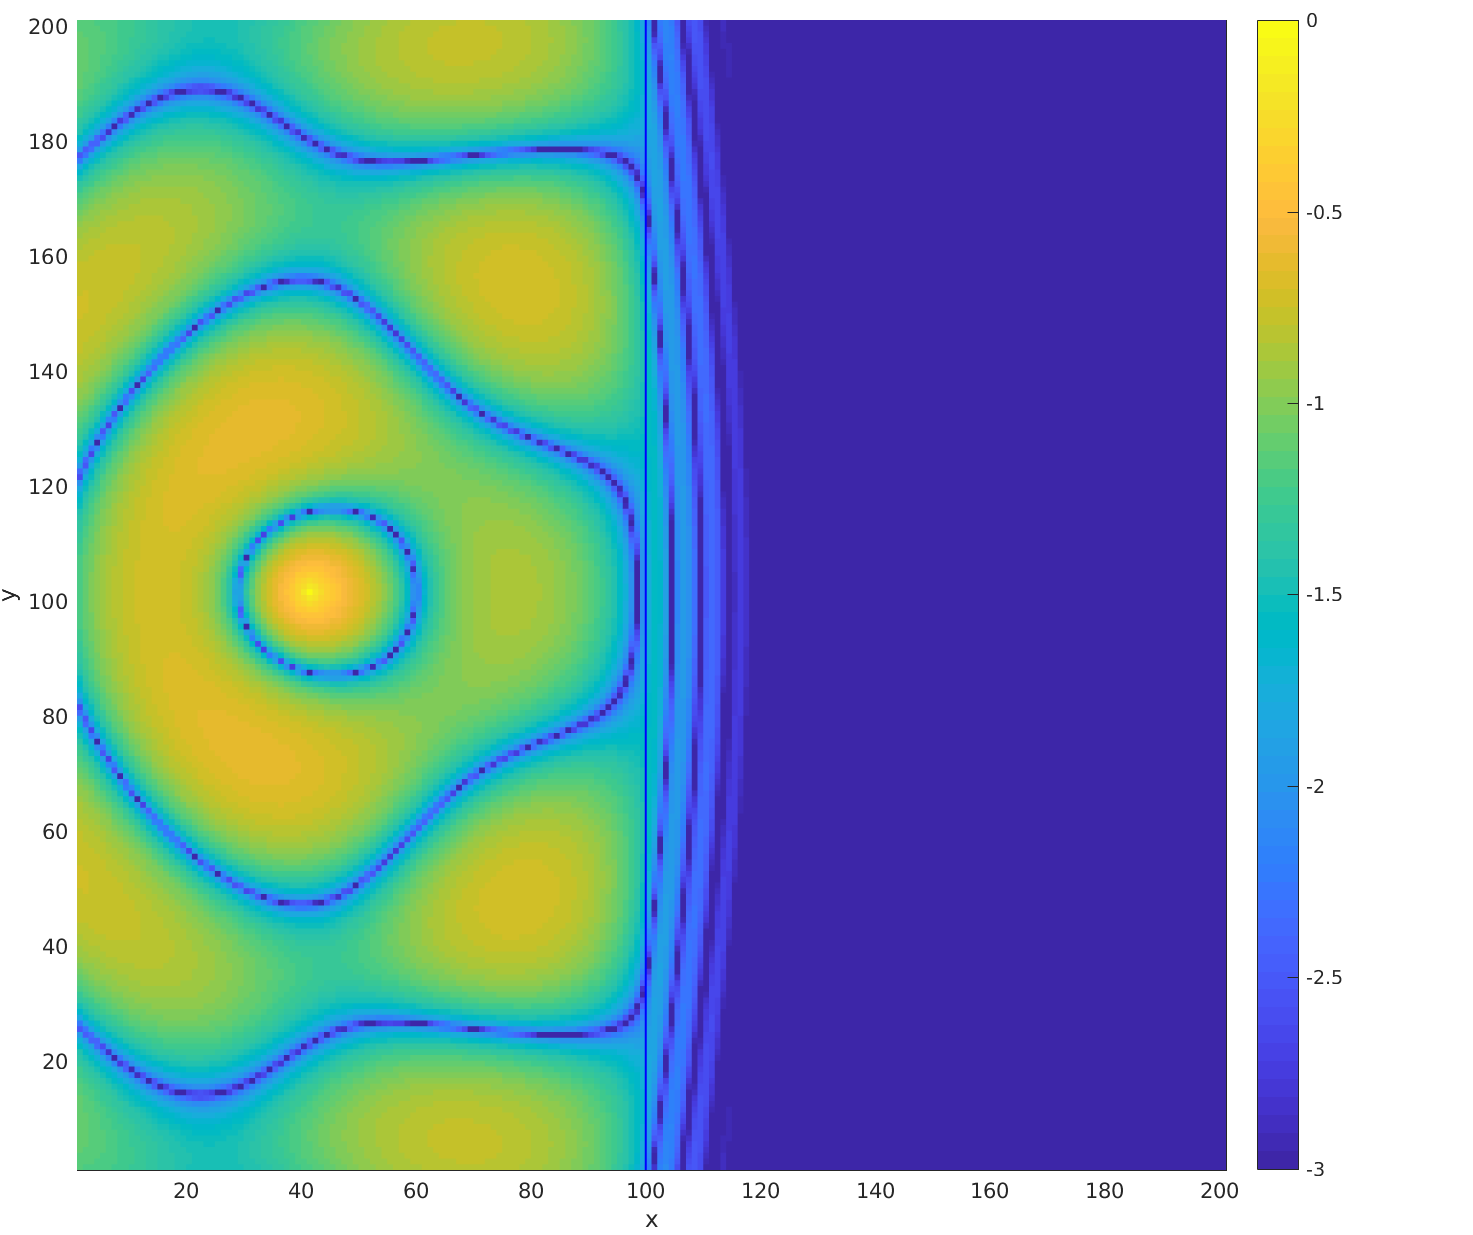
\includegraphics[width=.8\textwidth]{img/SAR_layer_im.pdf}
     \caption{Decay of the wave amplitude in a lossy layer of cerebral tissue}
     \label{fig:valid:SAR_Layer}
\end{figure}
\begin{figure}[H]
\centering
    \includegraphics{img/SAR_Layer.tex}
     \caption{Wave propagation with a lossy layer of cerebral tissue}
     \label{fig:valid:SAR_Layer_x}
\end{figure}

Hence, the simulation is validated and more advanced simulations can be designed.
\end{document}